\section{Optional: Solder Some Gates}

If you have the time and equipment, it can be fun and useful to solder some of the components together to make some of the basic logic gates. Several completed PCBs are already available, so this exercise is optional. % Some of the more advanced gates and whole circuits will also be put on PCBs to make later experiments much less tedious.

\begin{figure}[h!]
\begin{center}
\fbox{
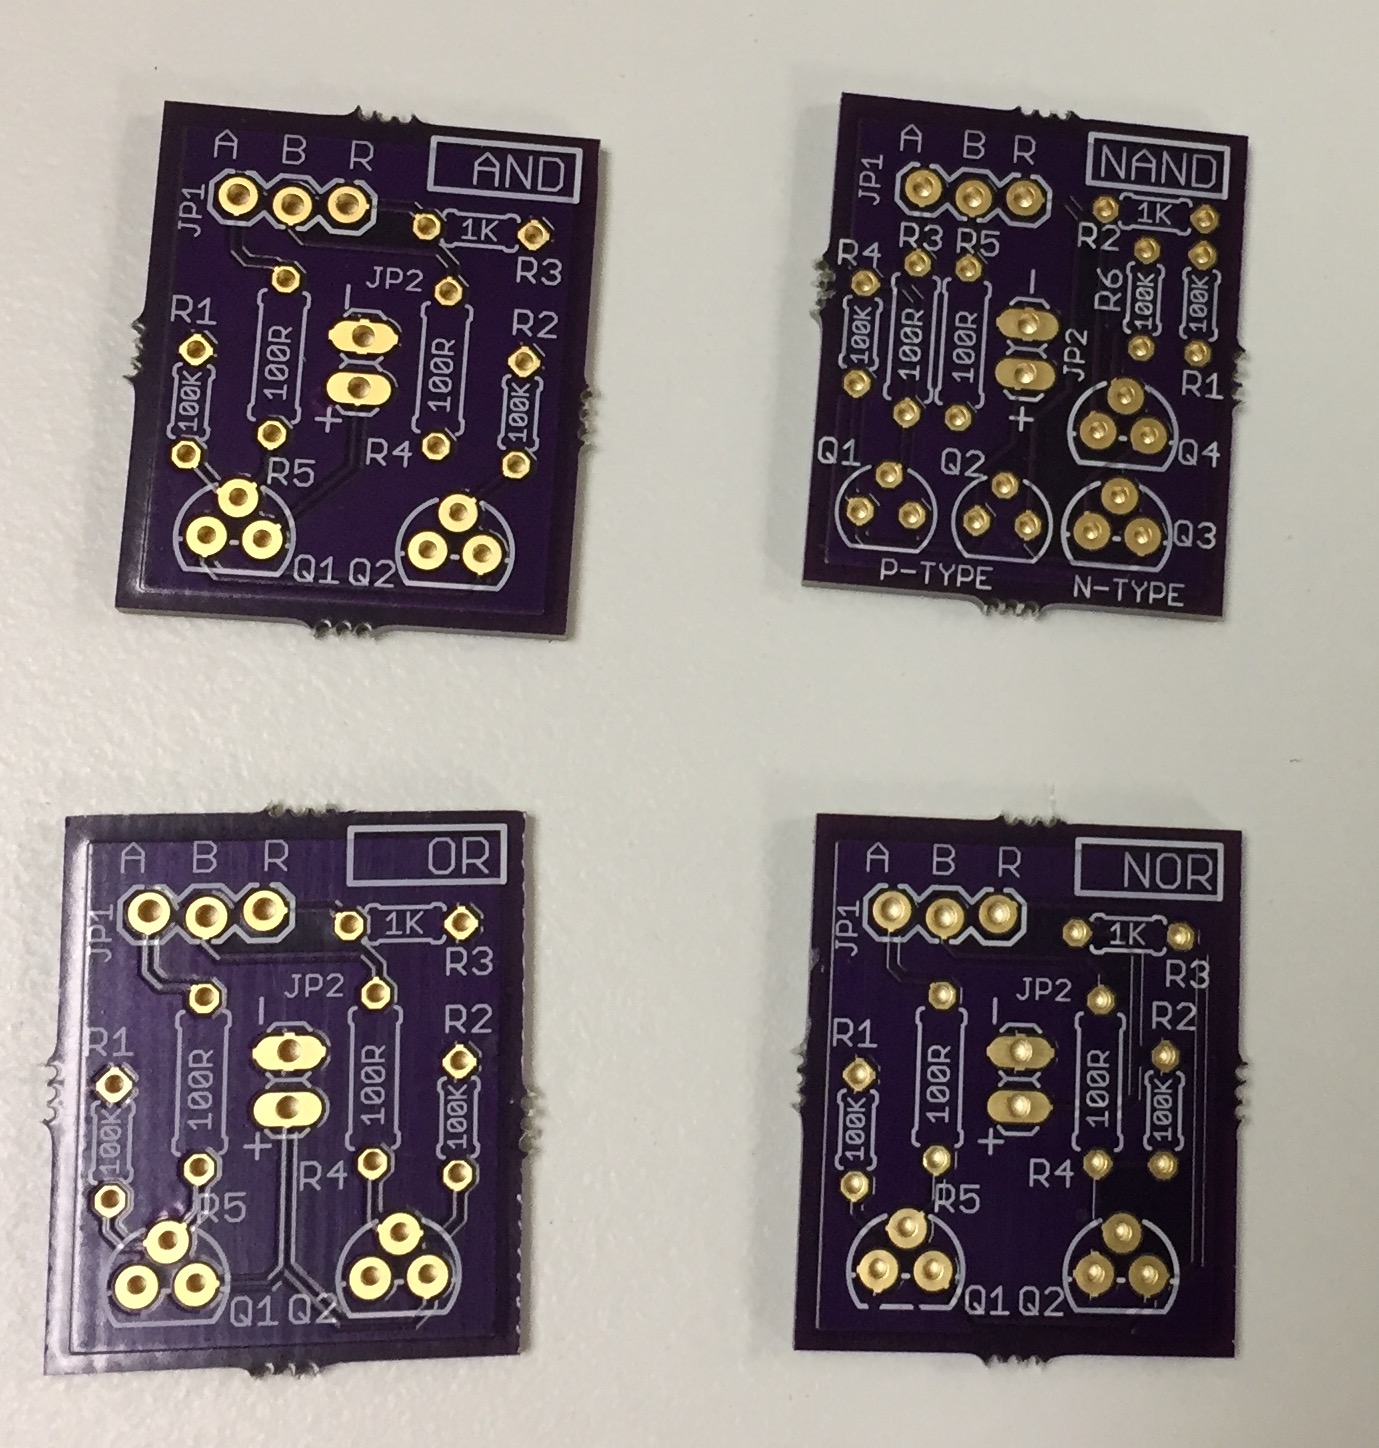
\includegraphics[scale=0.20]{barepcbs.jpg}
}
\end{center}
\caption{Four of the bare PCBs you will use when creating the gates. You will solder a set of specific components in the correct places, and then you will end up with the building blocks of computers.}
\label{fig:barepcbs}
\end{figure}

\subsection*{Solder An OR Gate}

\bi

\+ Get component list 
\+ Identify each resistor by color bands
\+ Read part numbers on the transistors to make sure (need magnifying glass)
%\+ Diodes (including LEDs) and transistors have a specific orientation so be sure to know which way things go
\+ solder resistors first
\+ then solder the transistors 
\+ lastly, solder the headers (note: use headers with long pins on both sides, to enable both breadboard use and discrete-wiring use)

\ei

